\documentclass[ignorenonframetext,aspectratio=169,10pt,xcolor=table]{beamer}

\definecolor{EnglishViolet}{HTML}{4B3D60}
\definecolor{Crimson}{HTML}{DB162F}

\beamertemplateshadingbackground{white}{white!80!black}
\setbeamercolor{structure}{fg=EnglishViolet}
\setbeamercolor{normal text}{fg=white!25!black}

\usefonttheme{structurebold}
\setbeamercolor{footnote}{fg=gray}
\setbeamercolor{alerted text}{fg=Crimson}
\setbeamerfont{alerted text}{series=\bfseries}
\beamertemplatenavigationsymbolsempty
\setbeamertemplate{footline}[frame number]
\setbeamertemplate{page number in head/foot}[appendixframenumber]
\setbeamertemplate{itemize items}[circle]

\usepackage{biblatex}
\addbibresource{references.bib}
\renewbibmacro{in:}{} % remove In
\renewbibmacro{title}{} % remove
\renewbibmacro{doi}{} % remove title

\newrobustcmd*{\footfullcitenomark}{%
  \AtNextCite{%
  \let\thefootnote\relax\let\mkbibfootnote\mkbibfootnotetext}%
\footfullcite}

\usepackage{graphicx}
\graphicspath{{figs/}}

\usepackage{tikz,pgfplots}
\usetikzlibrary{calc,shapes,positioning}
\pgfplotsset{compat=1.15}
\pgfkeys{/pgfplots/tuftelike/.style={
  semithick,
  tick style={major tick length=4pt,semithick,black},
  separate axis lines,
  axis x line*=bottom,
  axis x line shift=10pt,
  xlabel shift=5pt,
  axis y line*=left,
  axis y line shift=10pt,
  ylabel shift=5pt}}

\usepackage{menukeys}

\title{Scientific Imaging with ImageJ}
\author{J\'er\^ome Boulanger}
\date{June 23rd, 2022}

\begin{document}

\begin{frame}
  \maketitle
\end{frame}

\section{Introduction}

\begin{frame} \frametitle<presentation>{Introduction} The aim of this
  \only<presentation>{session}\only<article>{document} is to
  \begin{itemize}
  \item improve handling of scientific images for quantification and
    illustation,
  \item understand core concepts about images,
  \item discover ImageJ.
  \end{itemize} Online ressources are available here:
  \begin{itemize}
  \item \url{http://imagej.nih.gov}
  \item \url{https://imagej.net}
  \item \url{https://forum.image.sc}
  \end{itemize}
\end{frame}

\begin{frame} \frametitle{Context}
  \begin{block}{Quantification}
    \begin{itemize}
    \item Measure objects properties (intensity, area, shape, \dots)
    \item Count objects
    \item Relationship (co-occurrence, co-localisation), hierarchical.
    \item Speed, motion, \dots
    \end{itemize}
  \end{block}
  \begin{block}{Illustration}

    \begin{itemize}
    \item Use ImageJ to prepare the elements of a figure and import
      them in Illustrator.
    \item Relationship between markers
    \item Localisation of organelles
    \item Scale of objects
    \end{itemize}
  \end{block}
\end{frame}

\begin{frame} \frametitle{Image integrity} When preparing the figure:
  \begin{itemize}
  \item Apply adjustments to the entire image
  \item Track the sequence of manipulations (scripts/macro)
  \end{itemize} Include in the legend or methods section the following
  information:
  \begin{itemize}
  \item Equipment (microscopes/objective lenses, cameras, detectors,
    filters) and acquisition software used.
    % \begin{itemize}
    % \item[bad] Pictures were taken on the Zeiss\_780\_2S370.
    % \item[good] Images acquired on a Zeiss LSM 780 inverted
    microscope controlled by Zen black and equiped with a 63x/1.4 oil
    objective using a 488nm laser and GaAsp detectors.
    % \end{itemize}
  \item Time and space sampling (pixel size), image bit depth,
    temperature, imaging medium, fluorochromes
  \item Mention the look up table applied.
  \item Processing software and manipulations (deconvolution, 3D
    reconstructions, volume rendering, filtering, nonlinear operation,
    thresholding and projection).
  \end{itemize}
  \begin{center}
    Undocumented image manipulations can lead to accusations of research misconduct
  \end{center}

  \footfullcitenomark{nature-figs} \footfullcitenomark{ori-guidelines}
\end{frame}


\begin{frame} \frametitle{The ImageJ software}
  \begin{center} 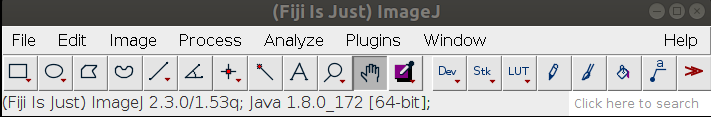
\includegraphics[width=0.5\textwidth]{ij}
  \end{center}
  \begin{itemize}
  \item ImageJ is a Java based image processing software.
  \item Java programs run on the java virtual machine (JVM)
  \item Can run on many operating system (Microsoft Windows, Mac OS,
    Linux, \dots)
  \item Developed by Wayne Rasband since 1997 at the National
    Institute of Health
  \item ImageJ eco-system
    \begin{itemize}
    \item ImageJ2: rewrite of ImageJ for multi dimensional data
    \item Fiji: image processing package built around ImageJ2
    \end{itemize}
  \end{itemize} \footfullcitenomark{ij2}
  \footfullcitenomark{schneider_nih_2012}
\end{frame}

\begin{frame} \frametitle{Installation \& Updating}
  \begin{block}{First Installation}
    \begin{itemize}
    \item Download Fiji from
      \url{https://imagej.net/software/fiji/downloads}.
    \item Unzip and save somewhere on your hard drive where default
      users have access.
    \item In Windows open the folder and double ckick on ImageJ-win64
      and create a shortcut.
    \end{itemize}
  \end{block}
  \begin{block}{Updating}
    \begin{itemize}
    \item To update ImageJ to the latest version \menu{Help > Update
        ImageJ}.
    \item To install/update plugins collections and manage update
      sites \menu{Help > Update}
    \end{itemize}
  \end{block}
\end{frame}

\begin{frame} \frametitle{Fiji.app folder content} The Fiji.app folder
  is organized into several subfolders:
  \begin{itemize}
  \item \directory{jars} : contains the main jar (eg ij-1.53q.jar) and
    extra java dependencies
  \item \directory{macros} : contains macros you installed and the
    \texttt{StartupMacros.fiji.ijm}
  \item \directory{plugins}: contains the jar (java artifacts) of the
    plugins
  \item \directory{scripts}: contains a few matlab scripts
  \item \directory{lut} : look up tables (mapping for intensity to
    displayed colors)
  \end{itemize}
\end{frame}

\begin{frame} \frametitle{Image is data}
  \begin{columns}
    \begin{column}{.6\textwidth}
      \begin{itemize}
      \item Sensors converts the number of detected photo-electrons
        into an electric volatage
      \item This voltage is then digitized into a number by the A/D
        converter.
      \item The image can be seen as an array of values with columns
        $x$ and rows $y$ starting at the top left corner at $(0,0)$.
      \end{itemize}
      \end{column}
    \begin{column}{.4\textwidth} \only<1>{
        \begin{tikzpicture}
          \begin{axis}[name=plot1,width=5.5cm,height=4.45cm,axis on
            top, enlargelimits=false, y dir = reverse, xlabel=x,ylabel=y] \addplot
            graphics[xmin=00,xmax=600,ymin=500,ymax=0] {array_img}; \draw[red,very
            thick] (axis cs:178,231) rectangle (axis cs:202,255);
          \end{axis}
        \end{tikzpicture} }
      \only<2>{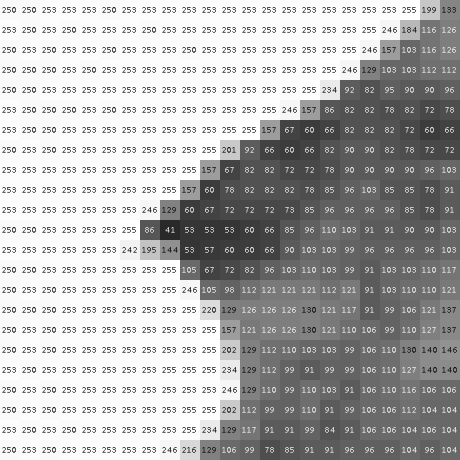
\includegraphics[width=\textwidth]{array_pixels}}
    \end{column}
  \end{columns}
\end{frame}

\begin{frame} \frametitle{General image formats}
  \begin{columns}
    \begin{column}{0.75\textwidth}
      \begin{itemize}
      \item Digital images can be saved from the volatile memory (RAM)
        of a computer to its persistent memory (HDD/SSD) as files with various
        formats.
      \item Most file formats include some sort of compression:
        \begin{itemize}
        \item Lossless compression (PNG): original values can be
          exactly retreived
        \item Lossy compression (JPEG): information is lost when
          storing the image
        \item Both (TIF): some formats are containers which can
          include various type of compression
        \end{itemize}
      \item ImageJ can read and write natively a few format such as
        TIFF, PNG, JPG
      \item Use TIF for saving intermediate results (with/without LZW
        compression) and PNG for figures
      \end{itemize}
    \end{column}
    \begin{column}{0.25\textwidth}
      
\includegraphics[width=\textwidth]{drive}
    \end{column}
  \end{columns}
\end{frame}


\begin{frame} \frametitle{Microscope vendor image formats} Each
  microscopy company has developed a format that can store multiple
  series with each a multi-channel multi-plane image stack.
  \begin{itemize}
  \item Zeiss
    \begin{itemize}
    \item LSM : TIF based file format with additional metadata and LZW
      compression
    \item CZI : JPEG-XR and Zstd lossless compressed image
    \end{itemize}
  \item Nikon
    \begin{itemize}
    \item ND2 : JPEG-2000 lossless compression
    \end{itemize}
  \item Leica
    \begin{itemize}
    \item LIF : Customized TIF file format
    \end{itemize}
  \item Olympus
    \begin{itemize}
    \item OIF: multi file formats with associated images in a folder
    \item OIB: store multiple OIF and dependent image in one file
    \end{itemize}
  \end{itemize} Some standardized image format have also been
  developed to increase inter-operability:
  \begin{itemize}
  \item OME-TIFF, OME-ZARR, ICS, HDF5
  \end{itemize}

\end{frame}

\begin{frame} \frametitle{Metadata}
  \begin {itemize}
  \item Metadata are essential to the interpretation and processing of
    the image
  \item Acquisition software collect additional information that are
    stored in the files
    \begin{itemize}
    \item Pixel size
    \item Spacing between z planes
    \item Detectors
    \item Objective
    \item Emission wavelength
    \item \dots
    \end{itemize}
  \item The Open Microscopy Environment (OME) defines a specification
    for storing data on biological imaging.
  \item Findable Accessibility, Interoperability, and Reusability
    (FAIR) principle.
  \end{itemize} \footfullcitenomark{ome-schema}
  \footfullcitenomark{fair}
  \footfullcitenomark{linkert_metadata_2010}
\end{frame}

\begin{frame} \frametitle{Loading an image}
  \begin{itemize}
  \item Fiji will detect supported file format when selecting
    \menu{File>Open} and use bioformat if needed to load an image from
    disk to memory.
  \item You can also use \menu{Plugins > Bio-Formats > Bio-Formats
      Importer} to use Bio-formats directly
  \item The Bio-Formats plugin remember previous settings, so use
    the tool directly to define the way the drag and drop or
    \menu{File>Open} behaves on non-native formats.
  \end{itemize}
\end{frame}

\begin{frame} \frametitle{Pixel size calibration \& scale bar}
  \begin{columns}
    \begin{column}{0.5\textwidth}
      \begin{itemize}
      \item Use \menu{Image>Properties\dots} to check and set the
        pixel size in each dimensions
      \item Use \menu{Analyze>Set Scale\dots} to use an known distance
        to set the scale
      \item Use \menu{Analyze>Tools>Scale Bar} to display the scale on
        a calibrated image
      \end{itemize}
    \end{column}
    \begin{column}{0.5\textwidth}
      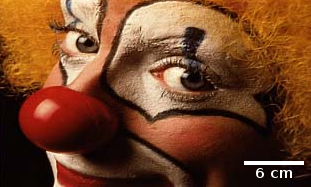
\includegraphics[width=\textwidth]{clown-scale}
    \end{column}
  \end{columns}
\end{frame}

\begin{frame} \frametitle{Quantization}
  \begin{columns}
    \begin{column}{0.7\textwidth}
      \begin{itemize}
      \item The intensity values are quantized into grey levels
      \item Images are saved as 8-bit or 16-bit images by acquisition
        software.
        \begin{itemize}
        \item For camera sensor (CCD, CMOS), photo-electron are
          accumulated in wells and converted into analogue voltages that are
          then digitized. Well depth is in the order of ~40000 electrons.
        \item For photo-multiplier tubes (PMT) photo-electrons are
          amplified using a chain of dynodes enabling to count individual
          photons.
        \end{itemize}
      \end{itemize}
      \begin{itemize}
      \item Use \menu{Image>Type>8-bit} to check \& convert an image
        to 8-bit, using the current dynamic range.
      \item 32-bit mode will allow to preserve the information if the
        intensities get out of the initial range.
      \end{itemize}
    \end{column}
    \begin{column}{0.3\textwidth}
      \begin{center} \small \rowcolors{1}{gray!25!bg}{white!25!bg}
        \begin{tabular}{cc}
          Bit depth & Dynamic range \\ \hline 8 &
          0-255 \\ 12 & 0-4095\\ 14 & 0-16383\\ 16 & 0-65535
        \end{tabular}
      \end{center}
    \end{column}
  \end{columns}
\end{frame}

\begin{frame} \frametitle{Brightness \& Contrast adjustment}
  \begin{itemize}
  \item \menu{Image > Adjust > Brightness \& Contrast...} or
    \keys{\Alt+\shift+C} launches the B\&C tool
  \item Pixels intensities are mapped linearly to the displayed
    intensity.
  \item Enable to discard unused part of the dynamic range
  \item Adjust the Minimum and Maximum of the dynamic range which will
    be displayed.
  \item Adjust the Brightness and Contrast to change how they are
    display.
  \item Press \menu{Auto} to stretch the intensities between a
    predefined percentage of saturated pixels. Equivalent to \menu{Process
      > Enhance Contrast...} with the normalized option left unticked.
  \item Press \menu{Apply} to change the pixel values.
  \item When changing the image mode (16-bit to 8-bit or 32-bit to
    8-bit) the B\&C settings are applied to the image.
  \end{itemize}
\end{frame}

%% \begin{frame} \frametitle{Brightness \& Contrast adjustment}
%%   \framesubtitle{Try it yourself}
%%   \begin{itemize}
%%   \item Open the boat example image \menu{File>Open Samples>Boats}
%%   \item Press the short cut \keys{\Alt+\shift+C}
%%   \item Change the minimum and maximum sliders and observe the image
%%   \item Press \keys{Set} and set the Minimum displayed value to 50
%%     and the maxium displayed value to 200, and press the \keys{OK} button.
%%   \item Finally press \keys{Apply} and obsere the change of the
%%     histogram in the B\&C window.
%%   \end{itemize}
%% \end{frame


\begin{frame} \frametitle{Histogram}
  \begin{itemize}
  \item Shows the frequency of each intensity values
  \item Use \menu{Analyze>Histogram} or \keys{\ctrl+h} to display the
    histogram
  \item Helps identify clipped values (under/over exposed, saturated)
  \item Visualise classes of pixels
  \end{itemize}
\end{frame}

\begin{frame} \frametitle{Look up table (LUT)}
  \begin{columns}
    \begin{column}{0.7\textwidth}
      \begin{itemize}
      \item Intensities are mapped to a color defined by a red, green
        and blue triplet value for display.
      \item Converting an image to RGB applies the current LUT
        (\menu{Apply LUT}, apply the B\&C settings)
      \item LUT can be inverted (black becomes white, \dots)
      \item Use LUT to help people with colour blindness
      \end{itemize}
    \end{column}
    \begin{column}{0.3\textwidth}
      \begin{center}
        \begin{tikzpicture}
          \begin{axis}[width=5cm,height=5cm,xlabel=Intensity,ylabel=Color,domain=0:255,axis
            x line=center, axis y line=center] \shade[left color=black,right
            color=white] (axis cs:0,0) rectangle (axis cs: 255,10); \shade[bottom
            color=blue,top color=red] (axis cs:0,0) rectangle (axis cs: 10,255);
            \addplot[structure,thick]{x}; \draw[thick,->] (128,15) -- (128,120);
            \draw[thick,->] (120,128) -- (15,128);
          \end{axis}
        \end{tikzpicture}
      \end{center}
    \end{column}
  \end{columns}
\end{frame}

%% \begin{frame} \frametitle{Look up table (LUT)} \framesubtitle{Try it
%%     yourself}
%%   \begin{columns}
%%     \begin{column}{0.7\textwidth}
%%       \begin{itemize}
%%       \item Open a grey scale image \menu{File>Open Samples>Boats}
%%       \item Apply a LUT to the image \menu{Image>Look Up Tables> 5
%%           Ramps}
%%       \item Convert the image to RGB \menu{Image>Type>RGB Color}
%%       \item Observe the values at each pixel
%%       \item Open the blobs example \menu{File>Open Samples>Blobs} and
%%         comment on the LUT
%%       \item Explore other commands \menu{Image>Color>Display LUTs},
%%         \menu{Image>Color>Edit LUT}
%%       \item Open the Fluorescent Cells sample and change the red channel
%%         to magenta.
%%       \end{itemize}
%%     \end{column}
%%     \begin{column}{0.3\textwidth}
%%       \begin{center}
%%         \begin{tikzpicture}
%%           \begin{axis}[width=5cm,height=5cm,xlabel=Intensity,ylabel=Color,%
%%             domain=0:255,axis x line=center, axis y line=center] \shade[left
%%             color=black,right color=white] (axis cs:0,0) rectangle (axis cs:
%%             255,10); \shade[bottom color=blue,top color=red] (axis cs:0,0)
%%             rectangle (axis cs: 10,255); \addplot[structure,thick]{x};
%%             \draw[thick,->] (128,15) -- (128,120); \draw[thick,->] (120,128) --
%%             (15,128);
%%           \end{axis}
%%         \end{tikzpicture}
%%       \end{center}
%%     \end{column}
%%   \end{columns}
%% \end{frame}

\begin{frame} \frametitle{Multi-channel images}
  \begin{itemize}
  \item Multi-channel images can be easily acquired by microcopes
    (multiple wavelength/fluorophores, brightfield/DIC, \dots)
  \item There are two types of color images:
    \begin{itemize}
    \item RGB images store color information into a single ($8 \times
      3$) 24 bit image
    \item Composite image are image whose channels are stored as
      individual (8,16-32-bit) image planes
    \end{itemize}
  \item On a composite image use \menu{Image>Color>Channel Tool} or
    \keys{\ctrl+\shift+z} to select the channel to display
  \item Create a multi channel image using \menu{Image>Color>Merge
      Channels\dots}
  \item Split channels of an image using \menu{Image>Color>Split
      Channels}
  \end{itemize}
%%  \begin{block}{Try it yourself}
%%     \begin{itemize}
%%     \item Open a composite image \menu{File>Open Samples>Fluorescent
%%         Cells}
%%     \item Use the channel tool to display each colour individually
%%     \end{itemize}
%%   \end{block}

\end{frame}

\begin{frame} \frametitle{Multi-dimensional images}
  \framesubtitle{Stack \& Hyperstacks}
  \begin{itemize}
  \item Images can have many dimensions (axis) associated to them
    channel c, time t, depth.
  \item Image stacks represent up to 4 dimensions (xyzc or xytc) with
    a maximum of 3 channels.
  \item Hyperstacks can have up to 5 dimensions xyzct with no limits
    on the number of channels.
  \item Virtual stacks enable to load only the images planes which are
    visualised.
  \end{itemize} To quickly visualize multi-dimensional data, use :
  \begin{itemize}
  \item Orthogonal views (\menu{Image>Stack>Orthogonal Views}) or
    \keys{\ctrl+\shift+H} can help visualize 3D data
  \item Maximum intensity projection \menu{Image>Stack>Z Project\dots}
  \item Reslice a stack with \menu{Image>Stack>Reslice\dots} or press
    \keys{/}
    % \item Extended depth of field: select the plane most in focus for
    each pixel. Activate the BIG-EPFL update site and search for
    ``Extended Depth Of Field''
    % \item 3D rendering
  \end{itemize} To synchronize two stacks use
  \menu{Analyze>Tools>Synchronize Windows}
\end{frame}

\begin{frame} \frametitle{Basic manipulation}
  \begin{itemize}
  \item Duplicate \keys{\ctrl+\shift+D} allows to crop, select
    channels and slices
  \item Use \keys{{+}} and \keys{-} or the magnifying glass tool to zoom
    in and out the displayed image.
  \item Use the hand tool to pan within a zoomed image.
  \item Changing the actual pixel size:
    \begin{itemize}
    \item \menu{Image>Scale} scale the image, if ``create a new
      image'' is not ticked, the image keep the same number of pixels and is
      cropped or padded as necessary.
    \item \menu{Image>Adjust>Size\dots} scale the image in place
      without cropping or creating a new image.
    \end{itemize}
  \item Use the search bar to look for tools.
  \end{itemize}
\end{frame}

\begin{frame} \frametitle{Selection / Region Of Interest (ROI)}
  \begin{itemize}
  \item Use the rectangle, circle, polygon, freehand, line tools to
    create selections.
  \item Use \menu{Edit>Selection>Specify} to enter manually the
    coordinate of a shape
  \item Transfer selection across images using
    \menu{Edit>Selection>Restore Selection} or \keys{\ctrl+\shift+E}
  \item Store selection into the ROI manager \menu{Edit>Selection>Add
      to manager} or \keys{t}
  \item Use \menu{Edit>Selection>Select None} \keys{\ctrl+\shift+A} to
    be sure no selection is active
  \item ROI from the ROI Manager can be stored as individual
    proprietary .roi file or as a collection into a .zip file.
  \item ROIs can be combined together using AND, OR, XOR logical
    operation
  \item Use \menu{Edit>Draw} and \menu{Edit>Fill} to set the pixel
    values on the contours resp. the inside of the shape to the value
    define by the colour picker tool.
  \end{itemize}
\end{frame}

\begin{frame} \frametitle{Threshold}
  \begin{itemize}
  \item Thresholding an image gives a binary image: 8-bit image with
    values either 0 or 255 whether the pixel intensity lies within two
    values (upper \& lower).
  \item Simplest form of image segmentation.
  \item Use the sort cut \keys{ctrl+\shift+T} to display the threshold
    tool.
    \begin{itemize}
    \item Use the sliders to set the upper and lower values
    \item Auto thresholds: Fiji includes a set of automatic threshold
      \footnote{\url{https://imagej.net/plugins/auto-threshold}}
    \item Stack histogram: the statistics will be computed on the all
      stack
    \end{itemize}
  \item Use \menu{Apply} or \menu{Process>Binary>Convert to mask} to
    apply the threshold and make the image binary.
  \item The menu \menu{Process>Binary>Make binary} will show a dialog
    if a threshold has been set.
  \item The LUT of binary images is inverted
  \end{itemize}
\end{frame}

\begin{frame} \frametitle{From thresholds to regions of interests}
  \begin{itemize}
  \item Use \menu{Edit>Selection>Create selection} to convert the
    threshold to a selection (can be a composite selection).
  \item Use the \menu{Analyze>Analyze Particles\dots} to convert
    connected components into individual ROIs and add them to the ROI
    Manager.
  \end{itemize}
%%  \begin{block}{Try it yourself}
%%     \begin{enumerate}
%%     \item Open the blob sample image
%%     \item Threshold the image
%%     \item Add connected components to the ROI Manager and get the
%%       number of blobs.
%%     \end{enumerate}
%%   \end{block}

\end{frame}

\begin{frame} \frametitle{Measurements}
  \begin{columns}
    \begin{column}{0.65\textwidth}
      \begin{itemize}
      \item Use \menu{Analyze>Set Measurements} to define the
        quantity to be measured
      \item Select an individual ROI and press \keys{\ctrl+M} to add
        measurements to the Result table.
      \item To measure the properties of all ROI stored in the ROI
        Manager, select them all with \keys{\ctrl+A} and press \menu{Measure}
      \end{itemize}
    \end{column}
    \begin{column}{0.35\textwidth}
      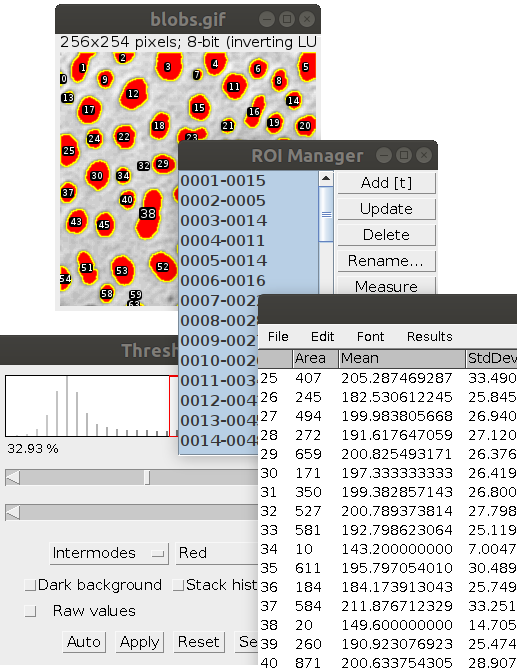
\includegraphics[width=\textwidth]{measure}
    \end{column}
  \end{columns}
\end{frame}

\begin{frame} \frametitle{Binary image processing} Binary image
  processing relies mostly on ``morphological image processing'' which
  process image by shapes. It can help refine the mask generated by
  thresholding:
  \begin{itemize}
  \item \menu{Process>Binary>Dilate} grow the masks, similar to
    \menu{Process>Filter>Maximum\dots}
  \item \menu{Process>Binary>Erode} shrink the masks, similar to
    \menu{Process>Filter>Minimum\dots}
  \item \menu{Process>Binary>Open} is equivalent to erode followed by
    dilate, removes small objects and lines
  \item \menu{Process>Binary>Close-} is equivalent to dilate followed
    by erode, bridge non touching objects etc
  \item \menu{Process>Binary>Watershed} separate touching objects
  \item \menu{Process>Binary>Fill Holes} will fill holes in the masks
  \end{itemize}
  \begin{center} 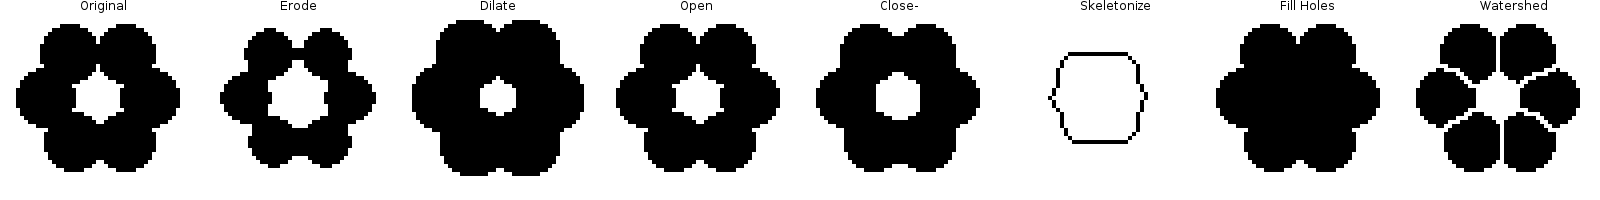
\includegraphics[width=\textwidth]{flower}
  \end{center}
\end{frame}

\begin{frame} \frametitle{Filtering} Image filtering can help reduce
  noise
  \begin{itemize}
  \item Box filtering \keys{\ctrl+\shift+S}
  \item Gaussian filtering \menu{Process>Filters>Gaussian Blur\dots}
  \item Median filtering \menu{Process>Filters>Gaussian Blur\dots}
  \end{itemize}

%%   \begin{block}{Try it yourself}
%%     \begin{itemize}
%%     \item Create an image with a light grey square on a darker grey
%%       square.
%%     \item Add noise to the image
%%     \item Launch the histogram and press \menu{Live}
%%     \item Apply some filtering to the image
%%     \item Apply a threshold
%%     \end{itemize}
%%   \end{block}
\end{frame}

\begin{frame} \frametitle{Background correction}
  \begin{columns}
    \begin{column}{0.5\textwidth}
      \begin{itemize}
      \item Background level can vary for several reason
        \begin{itemize}
        \item Uneven illumination
        \item Scattering
        \item Auto fluorescence
        \end{itemize}
      \item Simple generic correction
        \begin{itemize}
        \item Rolling ball from \menu{Process>Subtract Background\dots}
        \item Top Hat (image - grayscale opening) from
          \menu{Process>Filter>Top Hat\dots}
        \end{itemize}
      \item Illumination correction
        \begin{itemize}
        \item BASIC plugin
        \end{itemize}
      \end{itemize}
    \end{column}
    \begin{column}{0.5\textwidth}
      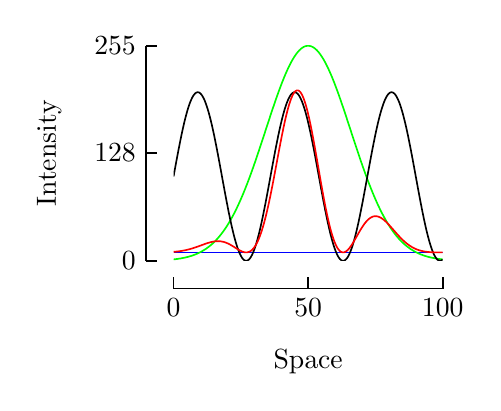
\begin{tikzpicture}
        \begin{axis}[tuftelike,
            domain=0:100,
            samples=200,
            no markers,
            ymin=0,ymax=255,xmin=0,xmax=100,
            xlabel=Space,ylabel=Intensity,
            width=5cm,
            ytick={0,128,255},xtick={0,50,100}]
          \addplot[blue] {10};
          \addplot[green] {255*exp(-0.002*(x-50)*(x-50))};
          \addplot[black] {100*(1+sin(10*x)};
          \addplot[red] {10+exp(-0.002*(x-50)*(x-50))*(100*(1+sin(10*x))};

        \end{axis}
      \end{tikzpicture}
    \end{column}
\end{columns}
\end{frame}

\begin{frame} \frametitle{Drift correction}
  \begin{itemize}
  \item Install Stackreg from the BIG-EPFL update site
  \item \menu{Plugin>Registration>Stackreg}
  \item The plugin can register drift using several motion models such
    as
    \begin{itemize}
    \item Translation
    \item Rigid body
    \item Rotation
    \item Scaled rotation
    \item Affine
    \end{itemize}
  \end{itemize}
\end{frame}

\begin{frame} \frametitle{Line profile}
  \begin{itemize}
  \item Line profile enable to measure distances visually.
  \item Draw a line and select \menu{Analyze>Plot Profile} or press
    \keys{\ctrl+K}
  \item Use \menu{Data>Add fit} to approximate the data with a model
  \end{itemize}
  \begin{center}
    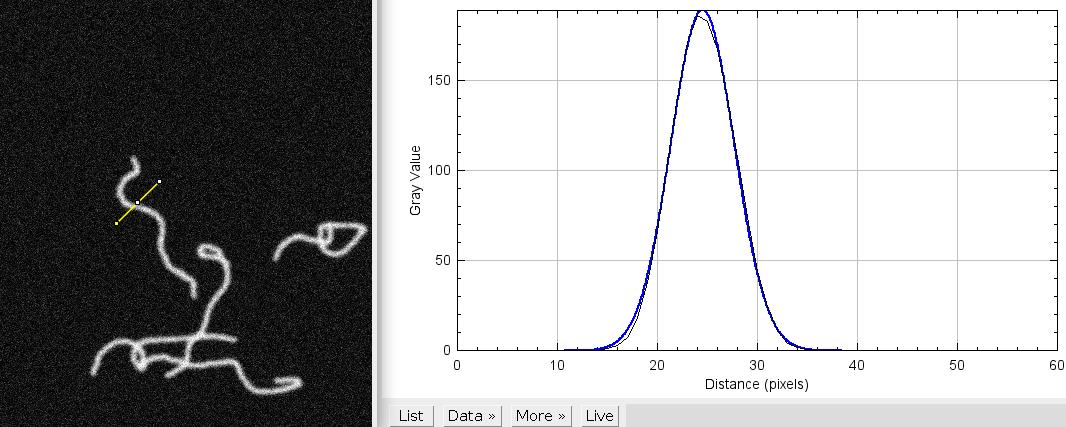
\includegraphics[width=0.75\textwidth]{line-profile}
  \end{center}
\end{frame}

\begin{frame} \frametitle{Kymograph}
  \begin{columns}
    \begin{column}{0.5\textwidth}
      \begin{enumerate}
      \item Create a maximum intensity projection
      \item Select lines using a freehand tool and add them to the ROI
        Manager
      \item Double click on the line tool to access the line width
        dialog
      \item Reslice the original stack
      \end{enumerate} Velocities can be then extracted from the
      kymographs using a macro for example.
    \end{column}
    \begin{column}{0.5\textwidth}
      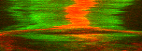
\includegraphics[width=\textwidth]{kymo_mito}
    \end{column}
  \end{columns}
\end{frame}

\begin{frame} \frametitle{Pixel classifier}
  \begin{itemize}
  \item Weka is a machine learning library in Java
  \item The weka plugin allows to annotate, train, export and apply
    the classifier
  \end{itemize}
  \begin{center} 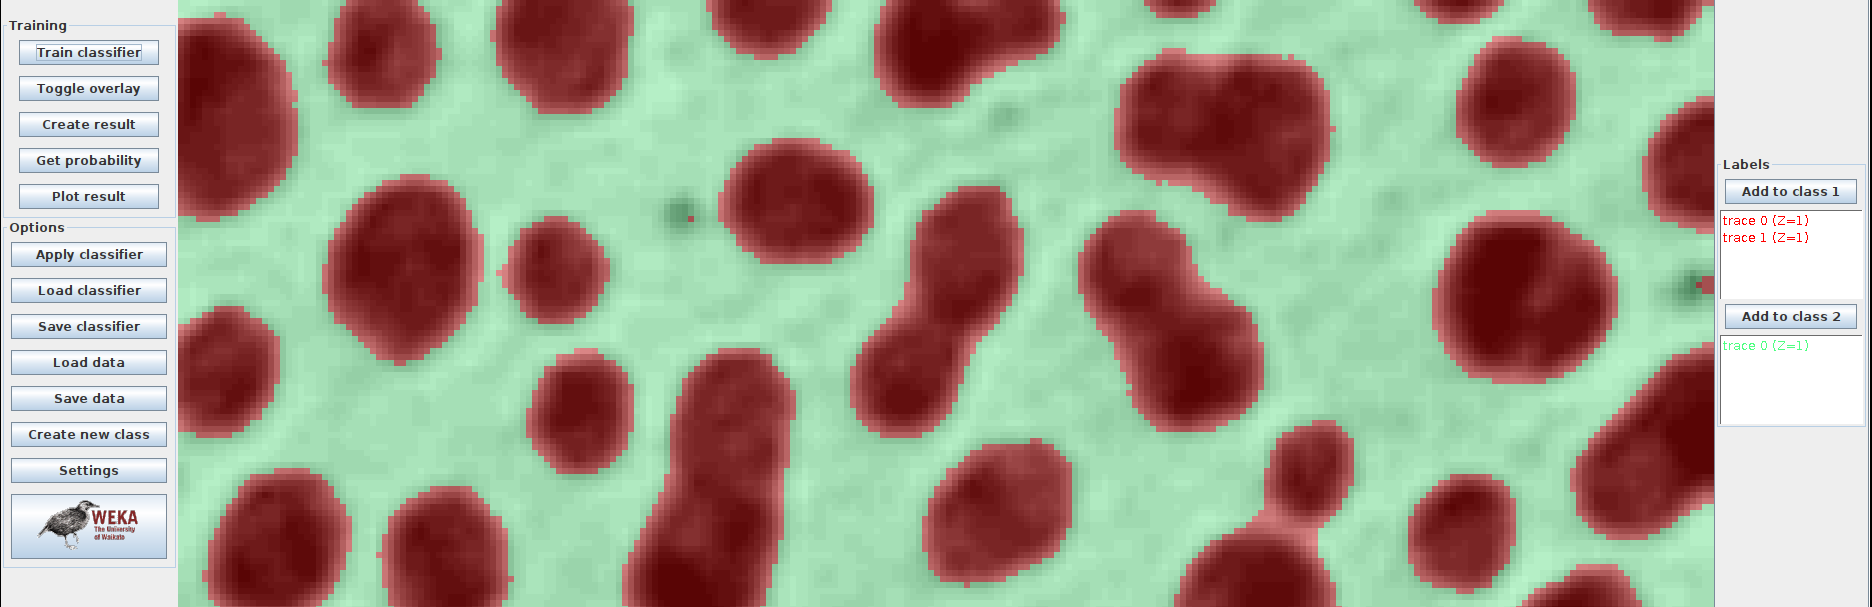
\includegraphics[width=0.75\textwidth]{weka}
  \end{center}
\end{frame}

\begin{frame} \frametitle{Nuclei segmentation with StarDist}
  \begin{itemize}
  \item StartDist is deep learning based approach based on star convex
    polygons
  \item It has been trained to identify cell nulcei.
  \item Install with \menu{Help>Update} and locate the StarDist and
    CSBDeep entries
  \item Launch trackmate from \menu{Plugins>StarDist}
  \end{itemize}
  \begin{center} 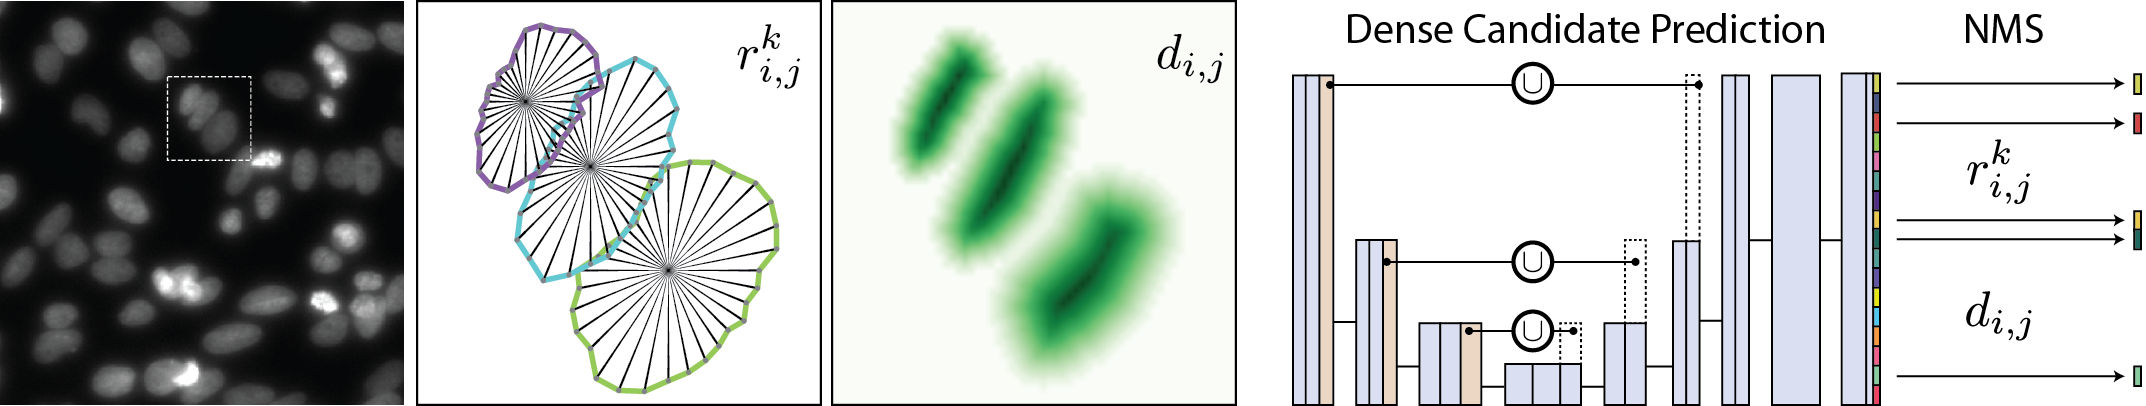
\includegraphics[width=0.75\textwidth]{stardist}
  \end{center}
\end{frame}

\begin{frame} \frametitle{Tracking with TrackMate}
  \begin{itemize}
  \item Detect spots and link them overtime
  \item Install trackmate using \menu{Help>Update} and locate the
    TrackMate entry
  \item Launch trackmate from \menu{Plugins>Tracking>Trackmate}
  \item Trackmate can also use stardist or weka for detecting objects
  \end{itemize}
  \begin{center} 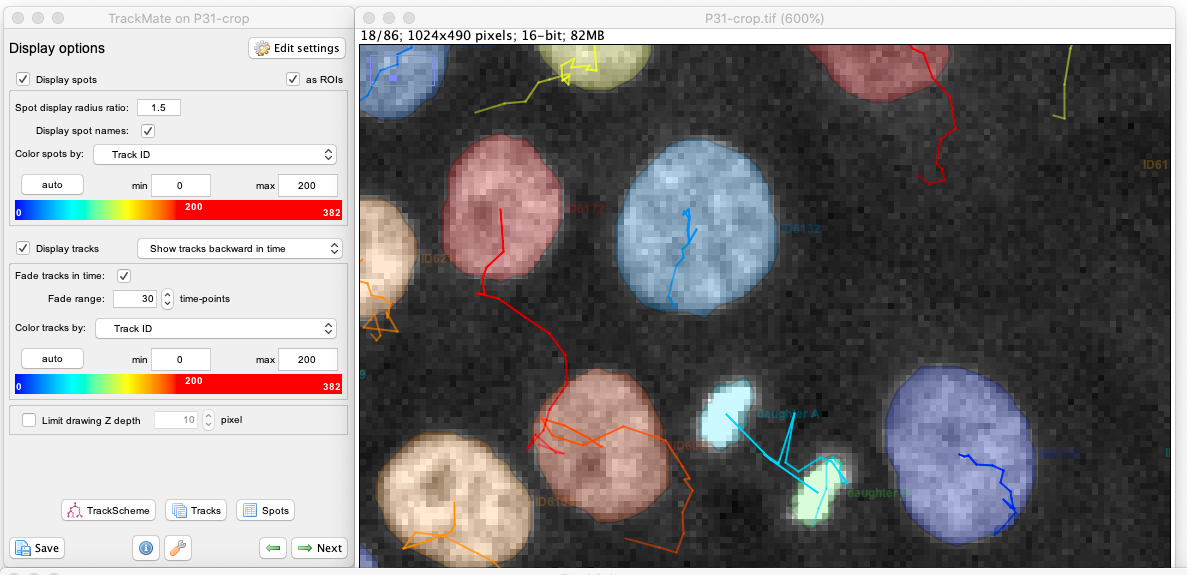
\includegraphics[width=0.5\textwidth]{trackmate}
  \end{center}
\end{frame}

\begin{frame} \frametitle{Basic quantification workflow}
  \begin{enumerate}
  \item Open the image
  \item Filtering
  \item Threshold
  \item Refine binary image
  \item Extract ROIs
  \item Measure
  \end{enumerate}
\end{frame}

\begin{frame} \frametitle{Basic figure preparation workflow}
  \begin{enumerate}
  \item Open the image
  \item Maximum intensity projection
  \item Adjust contrasts
  \item Convert to RGB
  \item Add a scale bar
  \item Export as PNG
  \end{enumerate}
\end{frame}

\begin{frame} \frametitle{Figure preparation tools}
  \begin{block}{Manually}
    \begin{itemize}
    \item Convert to RGB, add a scale bar without text, import in
      Illustrator
    \end{itemize}
  \end{block}
  \begin{block}{figureJ}
    \begin{itemize}
    \item Update sites IBMP-CNRS, ImageScience
    \end{itemize}
  \end{block}

  \begin{block}{EZFig}
    \begin{itemize}
    \item Update sites: EZF
    \end{itemize}
  \end{block}


  \begin{block}{QuickFigure}
    \begin{itemize}
    \item Update sites: QuickFigure
    \end{itemize}
  \end{block} \footfullcitenomark{mazo_plosone21}
\end{frame}

\begin{frame} \frametitle{Extension}

  ImageJ functionality can be extended and customised using:
  \begin{itemize}
  \item Macros (.txt, .ijm files)
  \item Scripts (Javascript, Python, Groovy \dots)
  \item Plugins (in Java)
  \end{itemize}
\end{frame}

\begin{frame} \frametitle{ImageJ Cheatsheet}
  \begin{columns}
    \begin{column}{0.5\textwidth}
      \begin{tabular}{ll}
        Image properties &\keys{\ctrl+\shift+P} \\
        Duplicate/crop & \keys{\ctrl+\shift+D} \\
        BrightnessContrast & \keys{\Alt+\shift+C} \\
        Channel Tools & \keys{\ctrl+\shift+Z} \\
        Add to ROI Manager & \keys{t} \\
        Restore Selection & \keys{\ctrl+\shift+E} \\
        Select All & \keys{\ctrl+A} \\
      \end{tabular}
    \end{column}
     \begin{column}{0.5\textwidth}
      \begin{tabular}{ll}
        Select None & \keys{\ctrl+\shift+A}\\
        Histogram & \keys{\ctrl+H} \\
        Orthoslices & \keys{\ctrl+\shift+H}\\
        Reslice & \keys{/} \\
        Threshold & \keys{ctrl+\shift+T} \\
        Measure & \keys{\ctrl+M} \\
        Smooth & \keys{\ctrl+\shift+S} \\
        Plot profile & \keys{\ctrl+K} \\
      \end{tabular}
    \end{column}
  \end{columns}

\end{frame}

\subsection{Good practice}

\begin{frame}{Data Management. The FAIR Guiding Principles} 
To be Findable:
\begin{itemize}
\item (meta)data are assigned a globally unique and persistent identifier
\item data are described with rich metadata (see below)
\item metadata clearly and explicitly include the identifier of the data it describes
\item (meta)data are registered or indexed in a searchable resource
\end{itemize}

To be Accessible:
\begin{itemize}
\item (meta)data are retrievable by their identifier using a standardized communications protocol
\begin{itemize}
\item the protocol is open, free, and universally implementable
\item the protocol allows for an authentication and authorization procedure, where necessary
\end{itemize}
\item metadata are accessible, even when the data are no longer available
\end{itemize}

\begin{flushright}
{\tiny \url{https://doi.org/10.1038/sdata.2016.18}}
\end{flushright}
\end{frame}

\begin{frame}{Data Management. The FAIR Guiding Principles} 
To be Interoperable:
\begin{itemize}
\item (meta)data use a formal, accessible, shared, and broadly applicable language for knowledge representation.
\item (meta)data use vocabularies that follow FAIR principles
\item (meta)data include qualified references to other (meta)data
\end{itemize}

To be Reusable:
\begin{itemize}
\item meta(data) are richly described with a plurality of accurate and relevant attributes
\begin{itemize}
\item (meta)data are released with a clear and accessible data usage license
\item (meta)data are associated with detailed provenance
\item (meta)data meet domain-relevant community standards
\end{itemize}
\end{itemize}

\begin{flushright}
{\tiny \url{https://doi.org/10.1038/sdata.2016.18}}
\end{flushright}

\end{frame}


\begin{frame}{Data Repositories} 
\begin{itemize}
\item FigShare ( \url{http://figshare.com}), 
\item Mendeley Data ( \url{https://data.mendeley.com/}), 
\item Zenodo ( \url{http://zenodo.org/}), 
\item DataHub ( \url{http://datahub.io}), 
\item IDR ( \url{https://idr.openmicroscopy.org/}) etc.
\end{itemize}

\vspace{1cm}
More info:
{\tiny
\begin{itemize}
\item \url{https://osc.cam.ac.uk/open-research/data-management-sharing},
\item  \url{https://www.data.cam.ac.uk}, 
\item \url{https://plos.org/open-science/open-data}
\end{itemize}
}
\end{frame}

\begin{frame}{Software good practice} 

\begin{itemize}
	\item Use meaningful variable and function names
	\item Write comments, documentation. Provide usage examples.
	\item Use a publicly accessible repository with version control. \\
	 (GitHub, GitLab,Bitbucket...). Add a license.\\
	It helps: 
	\begin{itemize}
	\item to track changes in your software
	\item collaborations 
	\item reproducibility of results 
	\item reusability
	\item to improves software quality. 
	\end{itemize}


	\item Register code in a community registry, making it easy to find
	\item Enable citation of the software 
	\item Use a software quality checklist
\end{itemize}

\vspace{1cm}
\begin{flushright}
{\tiny \url{https://fair-software.eu},\\ 
\url{https://plos.org/open-science/open-code/}}
\end{flushright}
\end{frame}

\end{document}
